\clearpage

\appendix

\renewcommand{\thesection}{\Alph{section}}
\renewcommand{\thefigure}{\Alph{section}.\arabic{figure}}
\setcounter{figure}{0}

\section{Apendix}

\subsection{Debugging \LaTeX\ integration with LANS}
\label{appendix:A}

LANS generates graphical output (images and graphs) in an EPS format and then uses the program \ttt{epstopdf} to convert it to PDF. Furthermore, LANS uses the program \ttt{pdflatex} and several LaTeX packages to generate a~tagged PDF document containing a~graphical summary of the processed data. These programs and necessary packages are typically installed as part of the LaTeX distribution. Some packages may, however, be missing and need to be installed `by hand'. Use the following steps to test whether the conversion from EPS to PDF and compilation of the PDF output work on your computer.

\vskip2.5mm
\s{Download the \ttt{test\_latex.zip} file from the same location as \ttt{LANS} (e.g., from this \href{https://www.dropbox.com/sh/gyss2uvv5ggu2vl/AABViAmt9WHryEP_xZBrCG_La?dl=0}{Dropbox folder}, sub-folder \ttt{test\_LaTeX}) and unzip it somewhere on your disk.}

\subsubsection{Testing of EPS to PDF conversion}

\s{Search whether the executable \ttt{epstopdf} is installed (present) locally on your computer.}

\nnb{If it is not, do some internet searching to figure out how to install it. If it is installed, proceed with the following step to test it.}

\s{Open a~terminal (if you are using Linux of MacOS) or a command prompt (\ttt{cmd}, if you are using Windows), navigate to the folder \ttt{eps} (a~sub-folder of the folder where you unzipped the \ttt{test\_latex.zip} file), and enter the following command:
\vskip2.5mm
\quad \ttt{epstopdf 12C.eps}}

\nnb{If a~file called \ttt{12C.pdf} was generated in the same folder as the file \ttt{12C.eps}, then the conversion works fine on your computer. If not, you will need to do a little bit of investigation to make it work.}

\subsubsection{Testing of \TeX\ to PDF conversion}

\s{Open the \ttt{test\_outputG.tex} file in an editor that is part of the \LaTeX\ distribution (e.g., \ttt{TeXworks} or \ttt{texworks}). The file is located in the folder created by unzipping the \ttt{test\_latex.zip} file.}

\s{Compile it using \ttt{pdfLaTeX}. If you use \ttt{TeXworks}, this is best done by clicking on the green arrow in the top-left corner of the program window, next to \ttt{pdfLaTeX}.}

\nnb{If you succeed in generating the file \ttt{test\_outputG.pdf} in this way, then the \TeX\ to PDF conversion should also work in Matlab when using LANS.}

\nnb{If you have never used \LaTeX\ on your computer, some of the packages required at this point (e.g., \ttt{geometry.sty} or \ttt{adjustbox.sty}) may be missing. Typically, these packages will be installed \emph{automatically} when needed by the compilation process in step~5. When prompted to do so during the compilation process, select \ttt{`yes'}, or \ttt{`yes to all'}, to install the missing \LaTeX\ packages. If the automatic installation didn't work, you will need to do a~little bit of investigation to figure out how to install the missing packages and ultimately succeed in compiling the \ttt{test\_outputG.tex} file to PDF locally on your computer.} 

\nnb{Note that you will need to go through the process of installation of missing \LaTeX\ packages only once.}

\s{Contact \ttt{L . P o l e r e c k y @ u u . n l} if you experience problems or seem unable to make this work.}

%%%

\subsection{Hierarchical data structure implemented in LANS}
\label{appendix:B}

\begin{figure}[!h]
\centering
\caption{\label{fig2:data_organization}%
	Visualization of the hierarchical organization of raw and processed nanoSIMS data implemented in Look@NanoSIMS. The figure is shown on the next page. %
  \textbf{(A)} The root folder (\ttt{nanosims}) contains a~project-specific sub-folder (e.g., \ttt{GAP2017}), which contains sub-folders with data measured on different days (e.g., \ttt{2017-09-28-GAP2017}, \ttt{2017-10-09-GAP2017}). %
  The `day folder' contains \emph{multiple raw datasets} measured on that particular day (\ttt{im} or \ttt{im.zip} files). %
  When a particular raw dataset is processed and analyzed, the data is stored in a `dataset folder' with the \emph{same name} as the dataset (see red ``!''). %
  \textbf{(B)} The `dataset folder' contains files defining the processing steps, including alignment information (\ttt{xyalign}), definition and classification of regions of interest (\ttt{cells.mat} and \ttt{cells.dat}, respectively), preferences (\ttt{prefs.mat}), and a comprehensive summary of results exported in a PDF file (\ttt{OutputG.pdf}). %
  The `dataset folder' also contains sub-folders with output generated by LANS in different formats. %
    \textbf{(C)} The ROI-specific ion counts and ion count ratios (\ttt{dac} files) are stored in the \ttt{dat} folder. %
    \textbf{(D)} The images, graphs, histograms, etc., are stored in the \ttt{pdf} folder.}%
\end{figure}

\newpage
\begin{center}
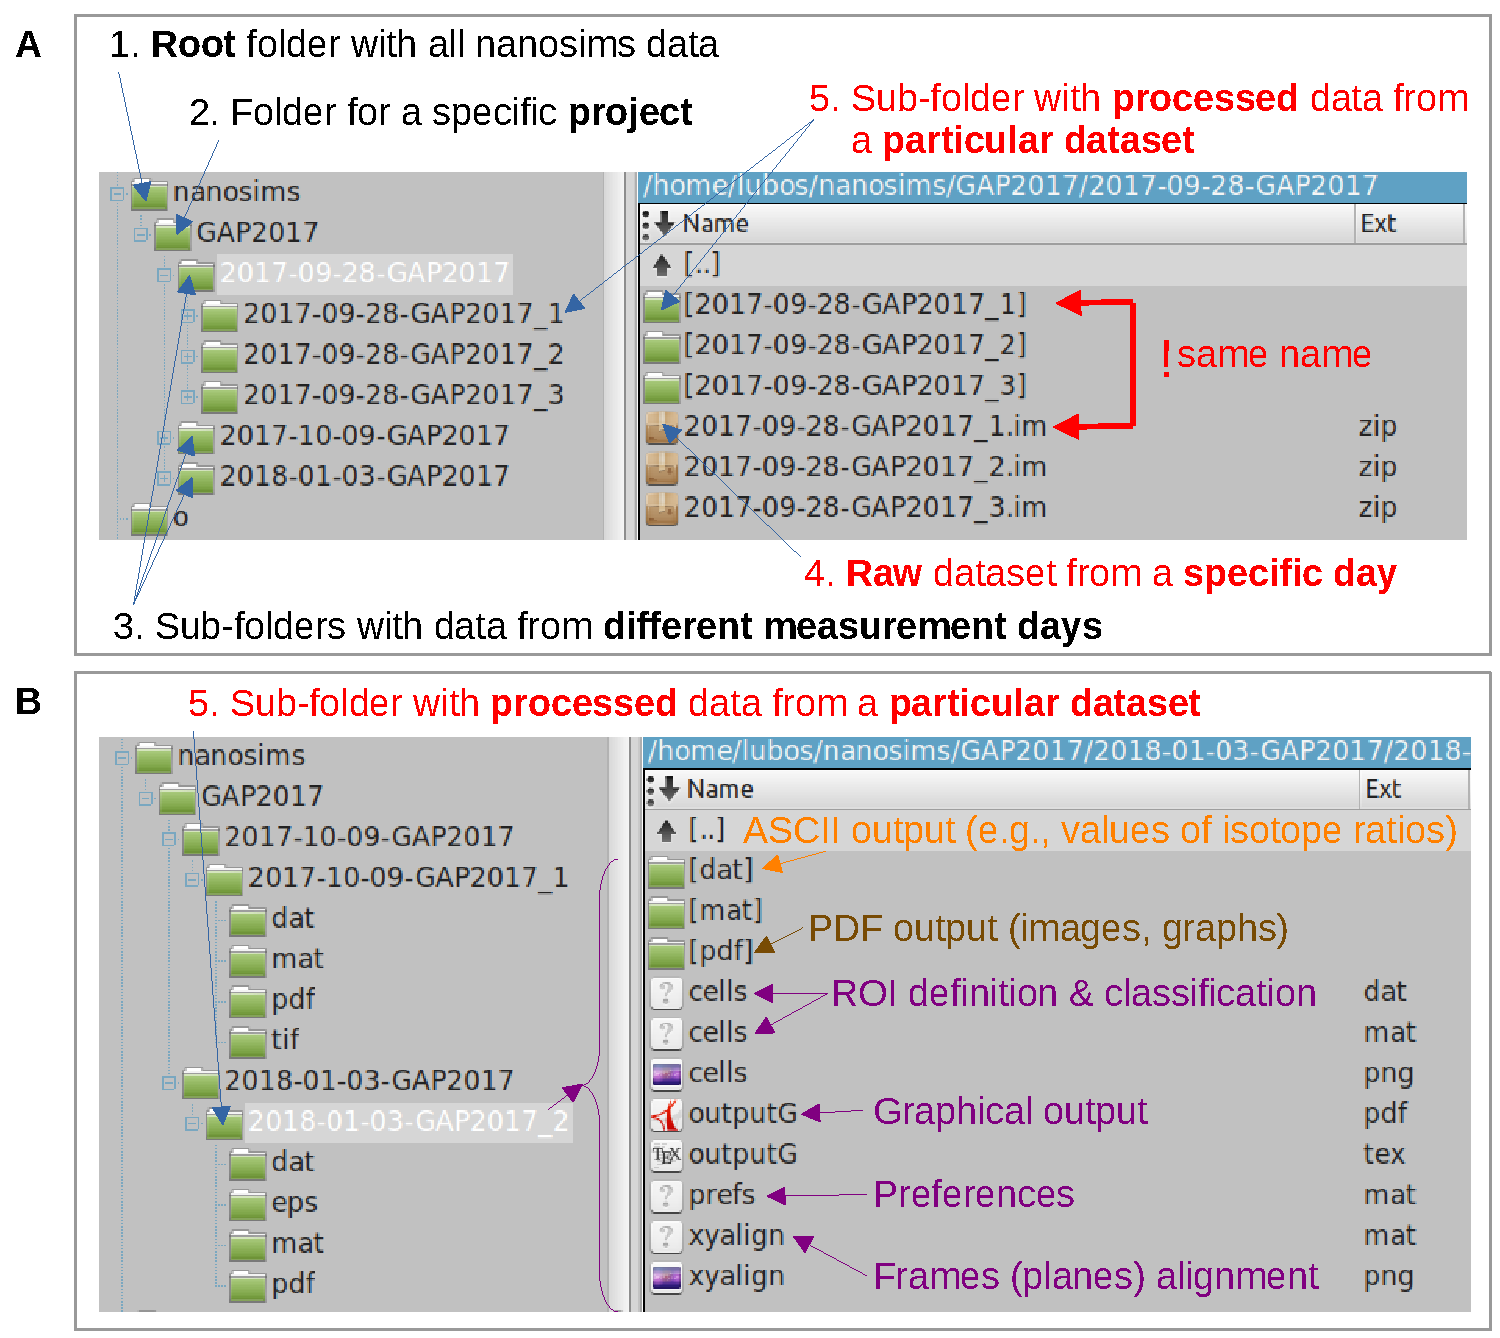
\includegraphics[scale=0.6]{figs2/folders_organizationAB}\\
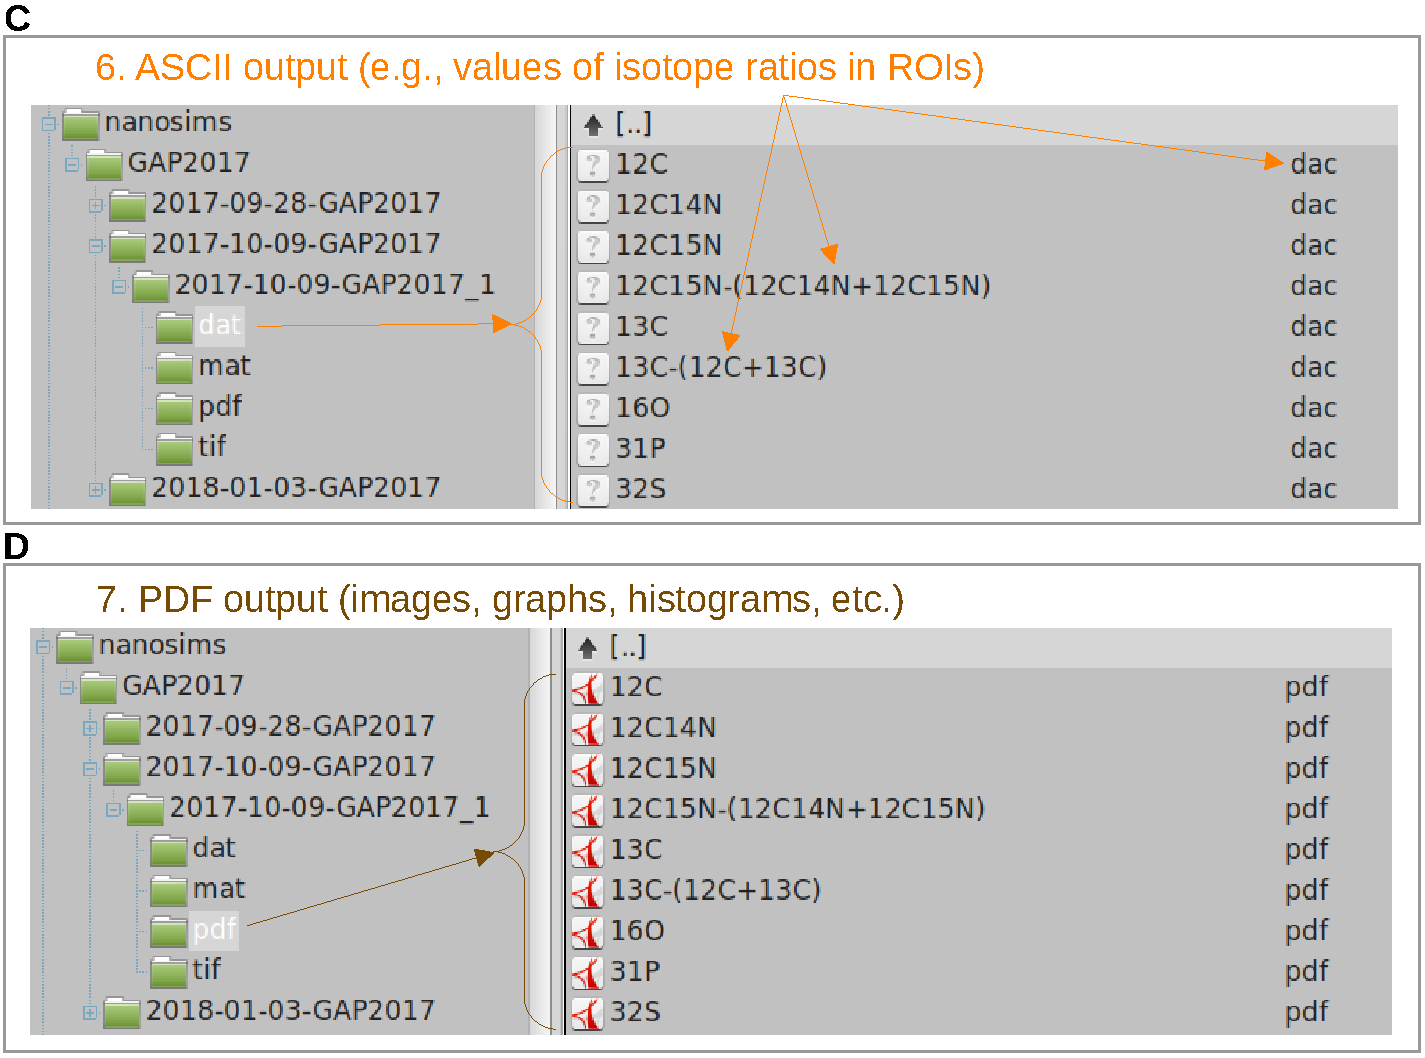
\includegraphics[scale=0.6]{figs2/folders_organizationCD}
\end{center}